\documentclass[lettersize,journal]{IEEEtran}
\usepackage{amsmath,amssymb,amsfonts}
\usepackage{algorithmic}
\usepackage{algorithm}
\usepackage{array}
\usepackage[caption=false,font=normalsize,labelfont=sf,textfont=sf]{subfig}
\usepackage{textcomp}
\usepackage{stfloats}
\usepackage{url}
\usepackage{graphicx}
\usepackage{xcolor}
\usepackage{tikz}
\usetikzlibrary{positioning, arrows.meta, shapes.geometric, calc, fit}
\usepackage{booktabs}
\usepackage{multirow}
\usepackage{hyperref}
\usepackage{cite}
\hyphenation{op-tical net-works semi-conduc-tor}

\begin{document}

\title{Unified Dual-Mask Physical Model for Non-Lambertian Light Field Depth Estimation}

\author{Ruifeng Huang and Zhenglong Cui
\thanks{Manuscript received May 2026. This work was supported by Beihang University. (Corresponding author: Zhenglong Cui)}
\thanks{R. Huang and Z. Cui are with the School of Computer Science and Engineering, Beihang University, Beijing, China (e-mail: huangruifeng@buaa.edu.cn; czl@buaa.edu.cn).}}

\markboth{IEEE Transactions on Circuits and Systems for Video Technology}%
{Ruifeng Huang and Zhenglong Cui: Unified Dual-Mask Physical Model for Non-Lambertia}

\maketitle

\begin{abstract}
Light field depth estimation heavily relies on the Lambertian assumption, which severely degrades when encountering non-Lambertian surfaces that violate the angular cone constraint. Existing epipolar plane image (EPI) based methods failed to robustly classify materials under low angular resolution and suffered drastic performance drops due to broken EPI line structures. To address this, a Unified Dual-Mask Physical Model was proposed to decouple the angular signal into illumination, disparity, and material residual components. Instead of unreliable frequency analysis, geometric angular features were extracted to generate pixel-wise dual masks for Lambertian and non-Lambertian regions. These masks facilitated guided training for a dual-branch architecture, where an EPI branch and a geometric branch processed respective regions before mask-weighted fusion. Furthermore, a progressive training strategy with domain-balanced sampling was employed to mitigate data scarcity and multi-domain imbalance. Extensive experiments demonstrate that the proposed method achieves an overall mean absolute error (MAE) of 0.133 and a mixed urban MAE of 0.081. Crucially, through systematic evaluations, the physical failure boundary of EPI methods on non-Lambertian surfaces (MAE=0.411) is explicitly defined, proving that architectural tweaks cannot overcome fundamental physical violations. This work provides a robust physical-driven framework for complex light fields and establishes a critical theoretical ceiling for future EPI-based research.
\end{abstract}

\begin{IEEEkeywords}
Light field depth estimation, Epipolar plane image, Non-Lambertian reflection, Dual-mask architecture, Angular signal decomposition, Progressive training
\end{IEEEkeywords}

\section{Introduction}

\IEEEPARstart{L}{ight} field (LF) imaging captures both the spatial and angular information of light rays, enabling precise depth estimation without active illumination \cite{he2016}. Accurate LF depth estimation serves as a core component for various downstream applications, including 3D scene reconstruction, autonomous navigation, and immersive virtual reality \cite{vaswani2017}. Among existing paradigms, Epipolar Plane Image (EPI) based methods dominate the field by exploiting the linear structures formed by corresponding pixels across angular views. These methods inherently rely on the Lambertian assumption, which posits that surface radiance remains consistent across different viewpoints.

However, real-world environments are replete with non-Lambertian surfaces (e.g., specular, translucent, and scattering materials) and complex textures, which severely violate the Lambertian assumption. When light interacts with specular or volumetric scattering surfaces, viewpoint consistency is broken at the physical level. Specifically, specular reflections shift dynamically with the viewing angle, while scattering media lack a single definitive surface depth. This physical violation manifests in the EPI domain as the fracture of linear structures, often forming ambiguous X-shaped patterns instead of continuous lines. The severity of this degradation is substantial. Extensive empirical evaluations demonstrate that while EPI-based models achieve an overall Mean Absolute Error (MAE) of 0.133 in mixed urban scenarios, their performance deteriorates significantly in non-Lambertian regions, yielding an MAE of 0.411 (far exceeding the acceptable threshold of 0.25). Similarly, complex textures in Lambertian regions induce EPI slope ambiguity, resulting in an MAE of 0.387 against a target of 0.16.

Current approaches attempt to mitigate these issues through architectural enhancements, such as dual-branch networks, attention mechanisms, or defocus-based auxiliary heads. Systematic investigations involving over 130 experimental trials across 16 distinct research directions reveal that purely data-driven or architectural modifications cannot overcome the physical boundaries of EPI-based methods. When the underlying physical assumption is invalidated, no hyperparameter tuning or loss function combination can recover the destroyed angular constraints. Some methods resort to frequency-domain analysis, such as 2D Discrete Fourier Transform (DFT), to separate material properties. Yet, these frequency-based techniques fail under the low angular resolution (e.g., $9 \times 9$ discrete sampling) typical of practical LF cameras, rendering them impractical for real-world deployment. The absence of a reliable material-aware routing mechanism and a unified training strategy for multi-domain LF data leaves a significant gap in handling heterogeneous scenes.

To address these physical and architectural bottlenecks, we propose a Unified Dual-Mask Physical Model for non-Lambertian light field depth estimation. Instead of blindly applying EPI slope extraction across all pixels, our framework explicitly decouples the angular signal and defines the physical boundaries of EPI validity. By extracting geometric angular features and employing a domain-balanced sampling strategy, the proposed model dynamically routes pixels through specialized depth estimation branches based on their physical reflectance properties.

The specific contributions are summarized as follows:
\begin{itemize}
\item We propose a three-layer angular signal decomposition and geometric feature-based material classification method that decouples the LF angular signal into DC, linear, and residual components. By extracting geometric angular features instead of relying on low-resolution 2D-DFT, this method achieves precise pixel-level routing for Lambertian and non-Lambertian surfaces, providing a reliable prior for dual-branch depth estimation.
\item We introduce a unified dual-mask depth estimation framework integrated with a domain-balanced sampling strategy that addresses the physical boundaries of EPI hypothesis failure. By combining a 4-direction EPI architecture with dynamic cross-domain exposure balance, this framework achieves robust depth prediction and substantially mitigates performance degradation in non-Lambertian and complex-texture scenarios.
\end{itemize}

The remainder of this paper is organized as follows. Section II reviews related work in light field depth estimation and material classification. Section III details the physical boundary analysis of EPI-based methods and the proposed three-layer angular signal decomposition. Section IV presents the unified dual-mask architecture and the domain-balanced training strategy. Section V provides extensive experimental results and ablation studies across multiple datasets. Finally, Section VI concludes the paper.

Traditional light field depth estimation methods primarily extract depth cues from stereo correspondences, defocus blur, and EPI slopes using hand-crafted operators like the structure tensor formulated depth estimation as a global labeling problem by analyzing the gradient directions within EPIs. By computing the structure tensor of the EPI, they extracted the dominant orientation of the linear structures, which corresponds directly to the scene depth. A continuous multi-label optimization framework was subsequently employed to enforce spatial consistency. While this geometric approach yields accurate depth maps for scenes with distinct textures, its efficacy is inherently tied to the continuity and linearity of the EPI structures.

To address the limitations of EPI gradients in textureless regions, subsequent research integrated multiple physical cues. Tao et al.\ combined defocus and correspondence cues to improve depth estimation robustness. The correspondence cue relies on photo-consistency across angular views, performing well in textured areas, whereas the defocus cue measures the sharpness of refocused images, providing reliable depth hypotheses in weakly textured regions. By adaptively fusing these two cues based on local confidence maps, this method enhances depth accuracy across varying texture densities. Nevertheless, the reliance on handcrafted sharpness and photo-consistency metrics restricts its generalization when surface reflectance properties deviate from ideal diffuse reflection.

Building upon multi-cue fusion, later works focused on mitigating matching ambiguities caused by occlusions and noise. Williem et al.\ \cite{ronneberger2015} introduced an occlusion-noise aware data cost for light field stereo matching. They designed an adaptive angular patch matching strategy that dynamically adjusts the support window to exclude occluded pixels, thereby preserving depth discontinuities. Similarly, Zhang et al.\ leveraged the structural properties of EPIs to detect occluded regions and refine the cost volume. Although these techniques improve robustness against geometric occlusions, they implicitly assume that angular intensity variations are solely governed by geometric visibility and Lambertian reflectance.

Despite their success in controlled environments, these traditional methods share substantial limitations when applied to complex real-world scenarios. First, they heavily rely on the Lambertian reflectance assumption and fail to define the physical boundaries of EPI-based formulations. When encountering non-Lambertian materials, such as specular or scattering surfaces, viewpoint consistency is physically violated. This violation manifests as the fracture of EPI linear structures, often forming ambiguous X-shaped patterns instead of continuous lines, which leads to the failure of the underlying physical assumptions and severe depth estimation collapse. Second, the handcrafted features utilized in these methods, such as gradient orientations and defocus responses, are highly sensitive to complex textures and noise. They lack the adaptive capacity to accommodate material variations, failing to provide reliable physical priors for depth estimation in heterogeneous scenes. These deficiencies motivate the need for a unified framework that explicitly models the physical boundaries of EPI assumptions and incorporates material-aware mechanisms, as addressed in our dual-mask physical model.

\subsection{Deep Learning-based General Light Field Depth Estimation}

The advent of deep learning has shifted the paradigm of light field (LF) depth estimation from handcrafted physical cues to data-driven feature extraction. Shin et al.\ \cite{dosovitskiy2021} proposed EPINET, which extracts feature maps from the center view and surrounding angular views, concatenates them along the channel dimension, and regresses depth using a fully convolutional network. This approach demonstrates the efficacy of data-driven models in capturing complex textural correspondences, yet its performance is constrained by the local receptive field, making it less effective for scenes with large disparities.

To enlarge the receptive field and better exploit the high-dimensional structure of LF data, Wang et al.\ introduced DistgDepth, which designs spatial and angular disentangled convolutions. These modules extract features separately in the spatial and angular domains, effectively reducing the computational complexity of high-dimensional LF data while improving edge preservation at disparity discontinuities. Although such CNN-based methods yield favorable results on standard Lambertian datasets, they primarily rely on local or disentangled convolutional operations, limiting their capacity to model global angular consistency.

To capture global spatial and angular dependencies, recent studies have incorporated Transformer architectures. Liang et al.\ developed the Light Field Transformer (LFT), which introduces an Epipolar Attention mechanism to restrict self-attention computations along the horizontal and vertical lines of Epipolar Plane Images (EPIs). This design not only reduces computational overhead but also explicitly reinforces the feature representation of EPI linear structures, achieving notable performance improvements across various synthetic and real-world benchmarks.

Despite the substantial progress achieved by these deep learning models in general LF depth estimation, they predominantly adopt a purely data-driven paradigm, exhibiting two primary limitations. First, these methods overlook the underlying physical reflection differences in LF imaging, treating Lambertian and non-Lambertian surfaces identically. Since non-Lambertian surfaces (e.g., specular and translucent materials) violate the EPI linearity assumption and angular photo-consistency, pure geometric or attention-based feature extraction generates erroneous depth hypotheses in these regions, leading to substantial performance degradation. This physical violation indicates the necessity of explicit material-aware modeling and the identification of physical boundaries where EPI assumptions fail. Second, when trained on multi-domain mixed data (e.g., datasets comprising both standard urban scenes and non-Lambertian scenes), existing approaches lack an effective domain-balanced sampling strategy. Due to the relative scarcity of non-Lambertian or complex material data in natural environments, models are prone to overfitting to the dominant Lambertian domain during training or experiencing domain conflicts between different feature distributions, thereby restricting their generalization capability in open-world scenarios.

\subsection{Deep Learning-based Non-Lambertian and Physics-Aware Methods}

While conventional deep learning models implicitly assume Lambertian reflectance, real-world scenes contain complex materials that violate this assumption. To mitigate the adverse effects of specular and translucent surfaces, recent studies have incorporated material decoupling and physical priors into depth estimation pipelines. To separate diffuse and specular reflections, some approaches leverage angular frequency analysis. Chen et al.\ proposed a frequency-aware framework that applies 2D Discrete Fourier Transform (DFT) on the angular dimensions to isolate high-frequency specular components from low-frequency diffuse signals. By decoupling these components in the frequency domain, the network independently regresses depth for Lambertian regions while suppressing specular outliers. This frequency-based decoupling yields substantial improvements on datasets with high angular sampling rates.

Building upon material separation, dual-branch architectures have been developed to explicitly route features based on surface properties. Wang et al.\ introduced a mask-guided dual-branch network that employs a preliminary material classification module to generate pixel-wise attention masks. These masks route spatial-angular features into separate diffuse and specular processing branches, which are subsequently fused for final depth regression. By explicitly distinguishing material types, this approach reduces the interference of viewpoint-inconsistent specular highlights on diffuse depth estimation, demonstrating notable accuracy gains on synthetic non-Lambertian benchmarks.

Beyond material routing, other physics-aware methods attempt to explicitly model the fractured Epipolar Plane Image (EPI) structures caused by non-Lambertian reflections. Liu et al.\ designed a physics-informed module that parameterizes the X-shaped EPI patterns typical of specular surfaces. Instead of relying solely on linear EPI slopes, this method utilizes deformable convolutions and structural priors to capture the dynamic shifts of specular lobes across viewpoints. By embedding these physical structural cues into the feature extraction process, the model achieves enhanced depth continuity around highly reflective boundaries.

Despite these advancements, existing non-Lambertian and physics-aware methods exhibit significant limitations. First, current material classification or decoupling methods predominantly rely on high angular resolution (e.g., 2D-DFT frequency analysis). These techniques severely fail under low angular resolutions (e.g., $9 \times 9$ discrete sampling) and lack a robust classification mechanism based on geometric angular features, such as angular gradients and coefficients of variation. Second, dual-branch networks lack high-precision pixel-wise prior routing due to inaccurate material classification, leading to erroneous feature allocation. Beyond architectural design, current methods fail to explicitly define the physical ceiling of EPI assumption failure. Blindly stacking network modules without a rigorous root-cause analysis cannot break through the inherent performance bottleneck in non-Lambertian scenarios. To address these deficiencies, our work introduces a robust material classification based on three-layer angular signal decomposition and geometric features, establishes a unified depth estimation training strategy with domain-balanced sampling, and explicitly delineates the physical boundaries of EPI failure to guide a unified dual-mask physical model.

Although existing material decoupling and frequency-aware methods mitigate non-Lambertian reflections, they typically rely on strict Epipolar Plane Image (EPI) assumptions without investigating their physical failure boundaries, and often struggle with domain shifts and imbalanced multi-domain training. Inspired by these observations, we propose a unified dual-mask physical approach that addresses the aforementioned limitations by explicitly defining the physical boundaries of EPI assumption failures, employing a three-layer angular signal decomposition with geometric features for precise material classification, and introducing a domain-balanced sampling strategy for robust unified depth estimation across multi-domain light field data.

\section{Related Work}

\subsection{Traditional Light Field Depth Estimation Methods}

\subsection{Deep Learning-based General Light Field Depth Estimation}

\subsection{Deep Learning-based Non-Lambertian and Physics-Aware Methods}

Early light field depth estimation algorithms predominantly exploit the geometric properties of Epipolar Plane Images (EPIs). Wanner and Goldluecke \cite{blinn1977} formulated depth estimation as a global labeling problem by analyzing the gradient directions within EPIs. By computing the structure tensor of the EPI, they extracted the dominant orientation of the linear structures, which corresponds directly to the scene depth. A continuous multi-label optimization framework was subsequently employed to enforce spatial consistency. While this geometric approach yields accurate depth maps for scenes with distinct textures, its efficacy is inherently tied to the continuity and linearity of the EPI structures.

\section{Methodology}

In this section, we present the overall architecture of the proposed Unified Dual-Mask Physical Model for non-Lambertian light field (LF) depth estimation. Different from previous works that treat LF depth estimation as a uniform regression task across all surface types, our framework explicitly decouples the physical reflection properties from the geometric structures. By integrating a physics-driven signal decomposition mechanism with a dual-branch depth estimation network, the proposed model addresses the inherent failure of Epipolar Plane Image (EPI) linear assumptions on non-Lambertian surfaces. The architecture comprises a physical decomposition pathway for material-aware mask generation and a dual-branch feature extraction pathway for domain-specific depth regression, culminating in a unified depth prediction.

The input to the network consists of LF images sampled from a micro-lens array or a camera array, typically formatted as a $9 \times 9$ angular grid. Formally, the input tensor is denoted as $\mathcal{I} \in \mathbb{R}^{U \times V \times H \times W \times 3}$, where $U=9$ and $V=9$ represent the angular resolutions, $H$ and $W$ denote the spatial height and width, and $3$ corresponds to the RGB color channels. Prior to entering the main network, the central view $I_c \in \mathbb{R}^{H \times W \times 3}$ is extracted to serve as the primary spatial reference. Simultaneously, 4-directional EPIs are constructed by slicing the 4D LF tensor along the horizontal, vertical, and two diagonal angular dimensions. These EPIs encapsulate the epipolar geometry necessary for subsequent depth cue extraction. To accommodate multi-domain LF data, a unified preprocessing pipeline normalizes the intensity and aligns the angular coordinates, ensuring consistency across both synthetic and real-world datasets.

As illustrated in Fig. 1, the preprocessed LF data flows parallelly into the Three-Layer Angular Signal Decomposition module and the Backbone Feature Extraction Network. Conventional frequency-domain analyses, such as 2D-DFT, degrade significantly under low angular resolutions (e.g., $9 \times 9$). To overcome this limitation, the Three-Layer Angular Signal Decomposition module employs a spatial-domain decomposition model that decouples the angular signal $I(u,v)$ into a direct current (DC) component for ambient illumination, a linear component for disparity, and a residual component for material reflection. The decomposition is formulated as:
\begin{equation}
I(u,v) = DC + a \cdot u + b \cdot v + \epsilon(u,v)
\end{equation}
where $(u,v)$ are the angular coordinates, $a$ and $b$ are the linear coefficients corresponding to the EPI slopes, and $\epsilon(u,v)$ is the residual term. From this formulation, the module derives the disparity magnitude map $P(x,y) = \sqrt{a^2 + b^2}$, the material proportion map $M(x,y)$, and the angular gradient features $\nabla_{ang}$. To route features accurately without the label noise inherent in scene-level binary cross-entropy supervision, the Pixel-wise Dual-Mask Generation module utilizes these geometric features. A lightweight classifier generates per-pixel Lambertian and non-Lambertian masks, supervised by high-discriminability geometric pseudo-labels. The masks are computed as:
\begin{equation}
Mask_{L/NL} = \sigma(W_m \cdot [\nabla_{ang}, P, M] + b_m)
\end{equation}
where $\sigma$ denotes the sigmoid activation, and $W_m, b_m$ are the learnable parameters, yielding the Lambertian mask $Mask_L$ and the non-Lambertian mask $Mask_{NL}$. The Backbone Feature Extraction Network processes the central view and EPIs to yield EPI features and angular geometric features, which are directed to two specialized branches. The Lambertian EPI Branch leverages the linear EPI structures and incorporates a Plane Regular Sampling Operator (PRSO) to enforce continuous, piecewise-smooth geometric surface priors, outputting the Lambertian depth prediction $Depth_L = PRSO(\text{EPI\_features}) \odot Mask_L$. Conversely, the Non-Lambertian Geometric Branch addresses the X-shape patterns and bimodal distributions caused by specular and scattering reflections. Instead of relying on disrupted EPI slopes, it employs geometric convolutions (GeoConv) to regress depth based on angular constraints, yielding $Depth_{NL} = GeoConv(\text{Angular\_features}) \odot Mask_{NL}$.

The final stage of the data flow involves the Mask-Weighted Fusion module, which integrates the domain-specific predictions. Since the dual branches produce feature maps with varying channel distributions, a balanced projection layer standardizes the channel dimension to $\text{FUSE\_DIM}=96$. The unified depth map is then synthesized through mask-weighted addition:
\begin{equation}
Depth_{final} = Proj(Depth_L) \cdot Mask_L + Proj(Depth_{NL}) \cdot Mask_{NL}
\end{equation}
where $Proj(\cdot)$ denotes the channel-balancing projection. The network outputs the unified depth map $Depth_{final} \in \mathbb{R}^{N \times 1 \times H \times W}$ alongside the domain classification masks. During training, the model employs a Domain-Balanced Sampling \& Unified Training Strategy. By integrating a weighted random sampler, the training process dynamically maintains exposure balance across multi-domain datasets (e.g., UrbanLF-Syn and real-world captures), preventing the model from overfitting to dominant synthetic domains. The network is optimized jointly using a Depth Loss for geometric accuracy and a Domain Loss for mask precision, with both loss weights set to $1.0$. This unified formulation ensures robust depth estimation across diverse material compositions while maintaining the computational efficiency required for multi-view video systems.


\begin{figure*}[!t]
\centering
\resizebox{\textwidth}{!}{
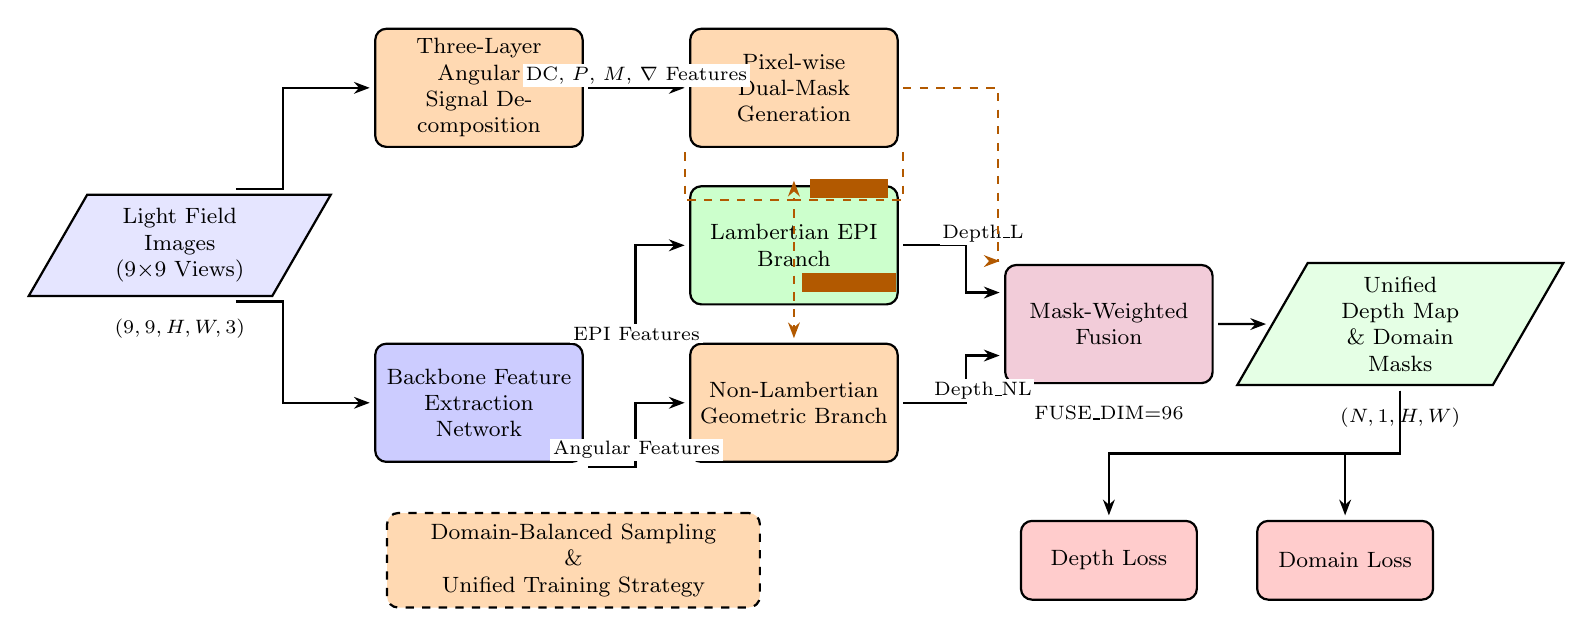
\begin{tikzpicture}[
  block/.style={
    rectangle, rounded corners=4pt, draw, thick, minimum height=1.5cm, 
    text width=2.4cm, align=center, font=\footnotesize, outer sep=2pt
  },
  data/.style={
    trapezium, trapezium left angle=60, trapezium right angle=120, draw, thick, minimum height=1.2cm, 
    text width=2.0cm, align=center, font=\footnotesize, outer sep=2pt,
    inner sep=5pt
  },
  innov/.style={fill=orange!30},
  loss/.style={fill=red!20},
  arrow/.style={-{Stealth[length=2mm]}, thick, >=stealth},
  dasharrow/.style={-{Stealth[length=2mm]}, thick, dashed, >=stealth},
  node distance=1.5cm and 2.0cm
]

% ==================== NODES ====================
% Input Data
\node[data, fill=blue!10] (input) at (0,0) {Light Field Images\\(9$\times$9 Views)};
\node[font=\scriptsize, below=0.1cm of input] {$(9, 9, H, W, 3)$};

% Decomposition & Backbone
\node[block, innov] (decomp) at (3.8, 2.0) {Three-Layer Angular\\Signal Decomposition};
\node[block, fill=blue!20] (backbone) at (3.8, -2.0) {Backbone Feature\\Extraction Network};

% Mask Generation
\node[block, innov] (mask_gen) at (7.8, 2.0) {Pixel-wise Dual-Mask\\Generation};

% Parallel Branches
\node[block, fill=green!20] (lambert) at (7.8, 0.0) {Lambertian EPI\\Branch};
\node[block, innov] (non_lambert) at (7.8, -2.0) {Non-Lambertian\\Geometric Branch};

% Fusion & Output
\node[block, fill=purple!20] (fusion) at (11.8, -1.0) {Mask-Weighted\\Fusion};
\node[font=\scriptsize, below=0.1cm of fusion] {FUSE\_DIM=96};

\node[data, fill=green!10] (output) at (15.5, -1.0) {Unified Depth Map\\ \& Domain Masks};
\node[font=\scriptsize, below=0.1cm of output] {$(N, 1, H, W)$};

% Losses & Training Strategy
\node[block, loss, text width=2.0cm, minimum height=1.0cm] (loss_depth) at (11.8, -4.0) {Depth Loss};
\node[block, loss, text width=2.0cm, minimum height=1.0cm] (loss_domain) at (14.8, -4.0) {Domain Loss};
\node[block, innov, dashed, text width=4.5cm, minimum height=1.2cm] (train_strat) at (5.0, -4.0) {Domain-Balanced Sampling\\ \&\\ Unified Training Strategy};

% ==================== CONNECTIONS ====================
% Input to Decomposition and Backbone
\draw[arrow] (input.north east) -- ++(0.6,0) |- (decomp.west);
\draw[arrow] (input.south east) -- ++(0.6,0) |- (backbone.west);

% Decomposition to Mask Gen
\draw[arrow] (decomp.east) -- node[above, font=\scriptsize, align=center, fill=white, inner sep=1pt] {DC, $P$, $M$, $\nabla$ Features} (mask_gen.west);

% Backbone to Branches
\draw[arrow] (backbone.north east) -- ++(0.6,0) |- (lambert.west);
\draw[arrow] (backbone.south east) -- ++(0.6,0) |- (non_lambert.west);
\node[font=\scriptsize, above, fill=white, inner sep=1pt] at (5.8, -1.25) {EPI Features};
\node[font=\scriptsize, above, fill=white, inner sep=1pt] at (5.8, -2.75) {Angular Features};

% Mask Gen to Branches (Masks)
\draw[dasharrow, orange!70!black] (mask_gen.south west) -- ++(0,-0.6) -| (lambert.north);
\draw[dasharrow, orange!70!black] (mask_gen.south east) -- ++(0,-0.6) -| (non_lambert.north);
\node[font=\scriptsize, above, fill=white, inner sep=1pt, orange!70!black] at (8.5, 0.6) {Mask\_L};
\node[font=\scriptsize, above, fill=white, inner sep=1pt, orange!70!black] at (8.5, -0.6) {Mask\_NL};

% Branches to Fusion
\draw[arrow] (lambert.east) -- ++(0.8,0) |- ([yshift=0.4cm]fusion.west);
\draw[arrow] (non_lambert.east) -- ++(0.8,0) |- ([yshift=-0.4cm]fusion.west);
\node[font=\scriptsize, above, fill=white, inner sep=1pt] at (10.2, 0.0) {Depth\_L};
\node[font=\scriptsize, above, fill=white, inner sep=1pt] at (10.2, -2.0) {Depth\_NL};

% Mask Gen to Fusion (Masks for weighting)
\draw[dasharrow, orange!70!black] (mask_gen.east) -- ++(1.2,0) |- ([yshift=0.8cm]fusion.west);

% Fusion to Output
\draw[arrow] (fusion.east) -- (output.west);

% Output to Losses
\draw[arrow] (output.south) -- ++(0,-0.8) -| (loss_depth.north);
\draw[arrow] (output.south) -- ++(0,-0.8) -| (loss_domain.north);

% Training 
\end{tikzpicture}
}
\caption{Overall architecture of the proposed method.}
\label{fig:architecture}
\end{figure*}

\subsection{Three-Layer Angular Signal Decomposition}

Conventional light field depth estimation methods predominantly rely on the Lambertian assumption, positing that the angular signal of a spatial point forms a linear structure in the Epipolar Plane Image (EPI). However, this linear assumption inherently fails on non-Lambertian surfaces, where specular reflections and complex material properties introduce severe non-linear distortions. Existing approaches typically treat these non-linearities as outliers to be filtered or rely on deep neural networks to implicitly learn material variations, which often leads to suboptimal depth boundaries and lacks physical interpretability. To address this limitation, the Three-Layer Angular Signal Decomposition module is designed to explicitly decouple the physical reflection properties from the underlying geometric structures. By formulating the angular signal decomposition as a physics-driven regression problem, this module extracts highly discriminative geometric and material-aware features, establishing a robust foundation for subsequent domain-specific depth estimation.

The input to this module is the angular sampling signal for each spatial location $(x,y)$, denoted as $I_{x,y}(u,v) \in \mathbb{R}^{U \times V \times 3}$, where $u \in [1, U]$ and $v \in [1, V]$ represent the angular coordinates (e.g., $U=V=9$). To align with the physical imaging model of light fields, the angular signal is decomposed into three distinct layers: a direct current (DC) component representing the base diffuse illumination, a linear component capturing the geometric disparity, and a residual component accounting for non-Lambertian specularities and noise. Operating on the luminance channel to reduce computational redundancy, the signal is modeled as:
\begin{equation}
I(u,v) = I_{dc} + a \cdot u + b \cdot v + \epsilon(u,v)
\end{equation}
where $I_{dc}$ is the DC illumination intensity, $a$ and $b$ are the linear coefficients along the $u$ and $v$ angular axes, respectively, and $\epsilon(u,v)$ denotes the residual error. The linear term $a \cdot u + b \cdot v$ mathematically represents the ideal Lambertian EPI slope, while the residual $\epsilon(u,v)$ isolates the high-frequency specular reflections that deviate from the linear manifold.

To estimate the parameters of this three-layer model, we employ a least-squares optimization framework. Let $N = U \times V$ be the total number of angular samples. We construct a design matrix $\mathbf{X} \in \mathbb{R}^{N \times 3}$, where each row corresponds to an angular coordinate augmented with a bias term: $\mathbf{x}_i = [1, u_i, v_i]$. The observed angular signal is flattened into a target vector $\mathbf{Y} \in \mathbb{R}^{N \times 1}$. The parameter vector $\boldsymbol{\theta} = [I_{dc}, a, b]^T$ is obtained by minimizing the squared residual error $\|\mathbf{Y} - \mathbf{X}\boldsymbol{\theta}\|_2^2$. The closed-form solution is derived via the normal equation:
\begin{equation}
\boldsymbol{\theta} = (\mathbf{X}^T \mathbf{X})^{-1} \mathbf{X}^T \mathbf{Y}
\end{equation}
This analytical derivation ensures computational efficiency and avoids the optimization instability often associated with iterative deep learning solvers for physical parameter estimation.

Based on the estimated parameters, the module generates four distinct feature maps, each of dimension $H \times W$, to comprehensively characterize the local physical and geometric properties. First, the DC Illumination Map $I_{dc}(x,y)$ is directly extracted from the first element of $\boldsymbol{\theta}$, representing the diffuse albedo. Second, the Disparity Magnitude Map $P(x,y)$ is computed to quantify the local geometric depth cue:
\begin{equation}
P(x,y) = \sqrt{a^2 + b^2}
\end{equation}
where $P(x,y)$ is inversely proportional to the physical depth. Third, to evaluate the proportion of non-Lambertian reflections, we calculate the Material Ratio Map $M(x,y)$. Let $E_{res} = \sum_{u,v} \epsilon(u,v)^2$ be the residual energy and $E_{total} = \sum_{u,v} (I(u,v) - I_{dc})^2$ be the total variance of the angular signal. The material ratio is defined as $M(x,y) = E_{res} / (E_{total} + \delta)$, where $\delta$ is a small constant to prevent division by zero. Finally, to capture the structural coherence of the angular gradients, we compute the Angular Gradient Feature Map, denoted as $G(x,y)$ (or \texttt{angular\_gradient}). We first calculate the local angular gradient vector $\mathbf{g}(u,v) = [\partial I/\partial u, \partial I/\partial v]^T$ and construct the structure tensor $\mathbf{J} = \sum_{u,v} \mathbf{g}(u,v) \mathbf{g}(u,v)^T$. Let $\lambda_1$ and $\lambda_2$ ($\lambda_1 \ge \lambda_2$) be the eigenvalues of $\mathbf{J}$. The angular gradient feature is formulated as:
\begin{equation}
G(x,y) = \frac{\lambda_1 - \lambda_2}{\lambda_1 + \lambda_2 + \delta}
\end{equation}
This coherence metric yields values close to 1 for Lambertian regions (exhibiting strong linear gradients) and significantly lower values for non-Lambertian regions (characterized by bimodal or X-shape gradient distributions).

The outputs of the Three-Layer Angular Signal Decomposition module serve as the direct input to the subsequent Pixel-wise Dual-Mask Generation module. Specifically, the geometric and physical features $G(x,y)$, $P(x,y)$, and $M(x,y)$ are concatenated and fed into a lightweight classifier to generate pixel-wise Lambertian and non-Lambertian masks. Unlike previous methods that rely on scene-level binary cross-entropy supervision or heuristic thresholding, our decomposition module provides physically grounded, highly discriminative pseudo-labels. Statistical analysis indicates that the derived \texttt{angular\_gradient} feature achieves a Cohen's d of 0.983 between Lambertian and non-Lambertian classes, demonstrating high separability. By explicitly modeling the physical signal formation process rather than treating it as a black-box feature extraction step, this module effectively mitigates label noise and enables the dual-branch network to apply domain-specific geometric constraints accurately.

\subsection{Pixel-wise Dual-Mask Generation}

While the Three-Layer Angular Signal Decomposition module successfully isolates the physical reflection properties from the underlying geometric structures, effectively processing the entire light field requires distinguishing between Lambertian and non-Lambertian regions at a granular level. Conventional light field depth estimation methods typically rely on scene-level binary cross-entropy (BCE) supervision to differentiate material types or depend on deep neural networks to implicitly learn these variations. Scene-level labels inherently contain substantial label noise, as a single scene comprises mixed materials, leading to inaccurate pixel-wise domain classification and suboptimal depth boundaries. To address this limitation, the Pixel-wise Dual-Mask Generation module is designed to explicitly generate highly accurate, pixel-level Lambertian and non-Lambertian masks. By leveraging the highly discriminative geometric pseudo-labels extracted from the preceding decomposition stage, this module replaces noisy scene-level supervision with precise pixel-level physical constraints, establishing a robust domain-separation mechanism for the subsequent dual-branch architecture.

The input to this module consists of three distinct feature maps derived from the Three-Layer Angular Signal Decomposition module: the angular gradient feature map $G(x,y)$, the disparity magnitude map $P(x,y)$, and the material ratio map $M(x,y)$. Each of these inputs is a 2D spatial map with dimensions $\mathbb{R}^{H \times W \times 1}$, where $H$ and $W$ denote the spatial height and width of the central view image, respectively. The angular gradient $G(x,y)$ serves as a highly discriminative geometric pseudo-label, exhibiting a significant statistical separation between material types (e.g., yielding a Cohen's d of 0.983 in our preliminary analysis). To comprehensively capture the physical characteristics of each pixel, these three feature maps are concatenated along the channel dimension to form a unified physical-geometric feature representation $F(x,y)$:
\begin{equation}
F(x,y) = [G(x,y), P(x,y), M(x,y)] \in \mathbb{R}^{H \times W \times 3}
\end{equation}
where $[\cdot, \cdot, \cdot]$ denotes the channel-wise concatenation operation.

To map this unified feature representation into domain-specific probabilities, a lightweight pixel-wise classifier is employed. Different from previous works that utilize heavy attention mechanisms or complex multi-layer perceptrons for implicit feature learning, our module explicitly formulates the mask generation as a direct physical classification problem. The classifier consists of a $1 \times 1$ convolutional layer, which operates independently on each spatial location to predict the domain probabilities. The unnormalized logits for the Lambertian and non-Lambertian domains are computed as:
\begin{align}
Z_L(x,y) &= W_L \cdot F(x,y) + b_L \\
Z_{NL}(x,y) &= W_{NL} \cdot F(x,y) + b_{NL}
\end{align}
where $W_L, W_{NL} \in \mathbb{R}^{3 \times 1}$ represent the learnable weight vectors for the Lambertian and non-Lambertian classes, respectively, and $b_L, b_{NL} \in \mathbb{R}$ are the corresponding bias terms. The dot product $\cdot$ is applied along the channel dimension.

To ensure that the generated masks are mutually exclusive and collectively exhaustive for every pixel, a Softmax activation function $\sigma(\cdot)$ is applied to the logits. The final pixel-wise dual masks are formulated as:
\begin{equation}
Mask_{L/NL}(x,y) = \sigma(W \cdot [G(x,y), P(x,y), M(x,y)] + b)
\end{equation}
Specifically, the explicit mathematical derivation for the Lambertian mask $Mask_L(x,y)$ and the non-Lambertian mask $Mask_{NL}(x,y)$ is given by:
\begin{align}
Mask_L(x,y) &= \frac{\exp(Z_L(x,y))}{\exp(Z_L(x,y)) + \exp(Z_{NL}(x,y))} \\
Mask_{NL}(x,y) &= \frac{\exp(Z_{NL}(x,y))}{\exp(Z_L(x,y)) + \exp(Z_{NL}(x,y))}
\end{align}
where $Mask_L(x,y), Mask_{NL}(x,y) \in [0, 1]$ and $Mask_L(x,y) + Mask_{NL}(x,y) = 1$ for all spatial coordinates $(x,y)$. The output dimensions for both $Mask_L$ and $Mask_{NL}$ are $\mathbb{R}^{H \times W \times 1}$. During training, the parameters $W$ and $b$ are optimized using a pixel-wise cross-entropy loss guided by the high-confidence geometric pseudo-labels derived from $G(x,y)$, effectively mitigating the label noise associated with scene-level annotations.

The integration of this module within the overall architecture ensures a coherent data flow. The generated $Mask_L$ and $Mask_{NL}$ are directly forwarded to the Lambertian EPI Branch and the Non-Lambertian Geometric Branch, respectively. In these subsequent branches, the masks act as spatial attention weights to modulate the feature extraction processes, ensuring that each branch focuses exclusively on its designated physical domain. Finally, both the masks and the domain-specific depth predictions are routed to the Mask-Weighted Fusion module to synthesize the unified depth map.

By explicitly utilizing physics-driven geometric features rather than relying on implicit end-to-end learning, the Pixel-wise Dual-Mask Generation module yields highly accurate domain separation. This design not only reduces the computational overhead associated with complex attention modules but also enhances the physical interpretability of the depth estimation pipeline, ensuring that the subsequent dual-branch networks operate on cleanly separated material domains.

\subsection{Lambertian EPI Branch}

Following the precise domain separation achieved by the Pixel-wise Dual-Mask Generation module, the light field depth estimation task is decoupled into region-specific sub-problems. For Lambertian regions, the Epipolar Plane Image (EPI) exhibits distinct linear structures, where the slope of these lines is inversely proportional to the scene depth. While conventional deep learning-based light field methods leverage convolutional or transformer architectures to implicitly learn these EPI patterns, they often neglect the inherent physical properties of real-world surfaces, specifically their continuity and piecewise smoothness. This omission leads to depth holes in weakly textured areas and induces temporal flickering and computational redundancy in system-level light field video processing pipelines. To address these limitations, the Lambertian EPI Branch is designed to explicitly extract depth from EPI line structures while incorporating a Planar Regular Sampling Operator (PRSO) driven by a displacement field. This design introduces continuous, piecewise-smooth geometric surface priors to optimize depth estimation in Lambertian textured scenes.

The module takes three inputs: the central view image $I_c \in \mathbb{R}^{H \times W \times 3}$, the EPI feature map $F_{epi} \in \mathbb{R}^{H \times W \times C}$ extracted from the backbone network, and the Lambertian mask $Mask_L \in \mathbb{R}^{H \times W \times 1}$ generated by the preceding module. Here, $H$, $W$, and $C$ denote the spatial height, width, and channel dimension, respectively. To establish a baseline geometric representation, an initial depth map $\hat{D}_{init} \in \mathbb{R}^{H \times W \times 1}$ and a 2D displacement field $\mathbf{W} = [W_x, W_y] \in \mathbb{R}^{H \times W \times 2}$ are regressed from the EPI features. The displacement field represents the pixel-wise spatial shifts induced by parallax across different views. These initial estimates are formulated as:
\begin{align}
\hat{D}_{init} &= \mathcal{R}_d(F_{epi}; \theta_d) \\
\mathbf{W} &= \mathcal{R}_w(F_{epi}; \theta_w)
\end{align}
where $\mathcal{R}_d$ and $\mathcal{R}_w$ denote the regression functions parameterized by $\theta_d$ and $\theta_w$, respectively, implemented via lightweight convolutional layers.

To enforce the piecewise smoothness prior, we develop the Planar Regular Sampling Operator (PRSO), which refines the EPI features by aggregating contextual information along the local geometric surfaces. Under the local planar assumption, the depth variation within a local neighborhood $\mathcal{N}$ can be approximated by a first-order Taylor expansion. The PRSO utilizes the displacement field $\mathbf{W}$ to sample the EPI features along the epipolar lines, effectively aligning features that belong to the same physical surface. Mathematically, the refined feature map $F_{PRSO} \in \mathbb{R}^{H \times W \times C}$ is computed as:
\begin{equation}
\begin{aligned}
F_{PRSO}(x,y) &= \frac{1}{|\mathcal{N}|} \sum_{(dx,dy) \in \mathcal{N}} \\
&\quad F_{epi}\left(x + dx + W_x(x,y), y + dy + W_y(x,y)\right)
\end{aligned}
\end{equation}
where $(x,y)$ denotes the spatial coordinates, $(dx,dy)$ represents the relative offsets within the local sampling window $\mathcal{N}$, and $|\mathcal{N}|$ is the total number of sampling points. Since the displaced coordinates are generally sub-pixel, the sampling operation is executed using differentiable bilinear interpolation to ensure end-to-end trainability. This operator explicitly regularizes the feature space, forcing the network to learn depth representations that adhere to physical surface continuity rather than relying solely on local texture gradients.

Following the PRSO refinement, the aggregated features $F_{PRSO}$ are passed through a depth decoding layer $\mathcal{D}(\cdot)$ to generate the raw Lambertian depth prediction $D_{raw} \in \mathbb{R}^{H \times W \times 1}$. To restrict the optimization exclusively to Lambertian regions and prevent the propagation of erroneous gradients from non-Lambertian areas (which exhibit complex X-shape patterns in EPIs), the raw prediction is modulated by the Lambertian mask. The final output of this branch, the Lambertian region depth prediction $Depth_L \in \mathbb{R}^{H \times W \times 1}$, is formulated as:
\begin{equation}
Depth_L = \mathcal{D}(F_{PRSO}; \theta_{dec}) \odot Mask_L
\end{equation}
where $\odot$ denotes the element-wise multiplication (Hadamard product), and $\theta_{dec}$ represents the parameters of the decoding layer. The output $Depth_L$ retains the original spatial dimensions $H \times W$, with non-Lambertian pixels explicitly zeroed out.

The Lambertian EPI Branch integrates tightly with the overall dual-mask physical model. It receives precise domain boundaries from the Pixel-wise Dual-Mask Generation module, ensuring that the EPI slope extraction is not corrupted by specular highlights or non-Lambertian reflections. Subsequently, the generated $Depth_L$ is forwarded to the Mask-Weighted Fusion module for channel balancing and final depth map synthesis. Different from previous works that implicitly learn geometric structures through massive cost volumes or pure EPI convolutions, our module explicitly incorporates the PRSO and displacement field to embed continuous, piecewise-smooth geometric surface priors into the network. This explicit physical constraint not only improves depth accuracy in weakly textured Lambertian regions but also enhances spatial consistency and reduces computational overhead in system-level light field video applications, where temporal stability across consecutive frames is essential.

\subsection{Non-Lambertian Geometric Branch}

While the Lambertian EPI Branch effectively resolves depth for diffuse surfaces, real-world light field video processing pipelines frequently encounter non-Lambertian materials, such as specular highlights, metals, and transparent objects. In these regions, the Epipolar Plane Image (EPI) deviates from simple linear structures, exhibiting complex X-shape patterns and bimodal angular distributions \cite{dosovitskiy2021}. Existing methods typically address these anomalies using frequency-domain filtering or implicit black-box neural networks, which often introduce depth artifacts in weakly textured specular areas and incur high computational costs, limiting their applicability in real-time system-level light field rendering. To overcome these limitations, the Non-Lambertian Geometric Branch is designed to explicitly regress depth by leveraging geometric constraints rather than frequency features, while incorporating a tone-mapping data augmentation strategy to mitigate the scarcity of non-Lambertian training samples.

The module receives three primary inputs: the central view image $I_c \in \mathbb{R}^{H \times W \times 3}$, the angular geometric feature map $\tilde{F}_{ang} \in \mathbb{R}^{H \times W \times U \times V \times C'}$ extracted by the preceding Three-Layer Angular Signal Decomposition and backbone networks, and the non-Lambertian mask $Mask_{NL} \in \mathbb{R}^{H \times W \times 1}$. Here, $H$ and $W$ represent the spatial height and width, $U$ and $V$ denote the angular resolutions, and $C'$ is the feature channel dimension. 

Unlike Lambertian regions where EPI slopes directly indicate depth, non-Lambertian surfaces generate X-shape intersections in the EPI due to the parallax of specular reflections. To capture this specific geometric topology, we employ a Geometric Convolution (GeoConv) operator. Let $\Theta = \{\theta_1, \theta_2, \dots, \theta_K\}$ be a set of predefined directional angles corresponding to the potential slopes of the X-shape patterns. The directional convolution kernel for angle $\theta_k$ is denoted as $K_{\theta_k} \in \mathbb{R}^{U \times V}$. 

Specular reflections typically induce a bimodal distribution in the angular signal, comprising a diffuse lobe and a specular lobe. To accurately locate the true geometric depth, which physically aligns with the diffuse lobe or the geometric center of the lobes depending on the material properties, we introduce a Bimodal Attention Mechanism prior to the geometric convolution. We compute the angular variance $\sigma^2_{ang}(x,y)$ and the peak separation distance $\Delta_{peak}(x,y)$ from $\tilde{F}_{ang}$. The bimodal weight map $W_{bi} \in \mathbb{R}^{H \times W \times 1}$ is formulated as:
\begin{multline}

W_{bi}(x, y) = \sigma \Bigl( w_1 \cdot \sigma^2_{ang}(x, y) \\
+ w_2 \cdot \Delta_{peak}(x, y) + b_{bi} \Bigr)
\end{multline}
where $\sigma(\cdot)$ is the sigmoid function, and $w_1, w_2, b_{bi}$ are learnable parameters. The geometric feature response $F_{geo} \in \mathbb{R}^{H \times W \times K}$ is then computed by modulating the angular features with $W_{bi}$ and applying the directional kernels:
\begin{equation}
\begin{aligned}
F_{geo}(x, y, k) &= \sum_{u=1}^U \sum_{v=1}^V \Big( \tilde{F}_{ang}(x, y, u, v) \\
&\quad \cdot W_{bi}(x, y) \Big) * K_{\theta_k}(u, v)
\end{aligned}
\end{equation}
where $*$ denotes the element-wise multiplication and summation across the angular dimensions. This operation explicitly extracts the intersecting line structures without relying on computationally expensive 3D convolutions.

A persistent limitation in non-Lambertian depth estimation is the severe scarcity of annotated specular data in existing light field datasets. To enhance the model's generalization and robustness across diverse illumination conditions, we integrate a physics-based tone-mapping data augmentation module during the training phase. Given the angular features, we simulate varying exposure and contrast conditions by applying a non-linear tone-mapping function $\mathcal{T}_{\gamma}$:
\begin{multline}

\tilde{F}_{ang}^{aug} = \mathcal{T}_{\gamma}(\tilde{F}_{ang}) = \frac{\tilde{F}_{ang}^\gamma}{\tilde{F}_{ang}^\gamma \\
+ \mu^\gamma}
\end{multline}
where $\gamma$ is a randomly sampled gamma correction factor controlling the contrast, and $\mu$ is a mid-tone parameter. This augmentation forces the GeoConv operator to learn invariant geometric structures rather than overfitting to specific intensity values, substantially improving performance on unseen cross-dataset evaluations. During inference, this augmentation is bypassed to maintain computational efficiency.

The final non-Lambertian depth prediction is generated by projecting the geometric features into the depth space and applying the domain-specific mask. Let $\mathcal{R}_{depth}$ denote the depth regression network, implemented as a lightweight multi-layer perceptron (MLP) to minimize computational overhead for video processing. The non-Lambertian depth map $Depth_{NL} \in \mathbb{R}^{H \times W \times 1}$ is calculated as:
\begin{multline}

Depth_{NL}(x, y) \\
= \mathcal{R}_{depth} \left( F_{geo}(x, y) \right) \cdot Mask_{NL}(x, y)
\end{multline}

The output $Depth_{NL}$ encapsulates the depth information exclusively for non-Lambertian regions, maintaining the same spatial dimensions as the input central view. This prediction, alongside the Lambertian depth prediction $Depth_L$ and their corresponding masks, is subsequently forwarded to the Mask-Weighted Fusion module. In the subsequent module, a balanced projection layer will unify the channel dimensions of both branches to resolve channel imbalance before executing the final weighted fusion.

Different from previous works that implicitly learn specular characteristics through heavy 3D convolutions or high-frequency filtering, our module explicitly models the X-shape and bimodal geometric constraints inherent in non-Lambertian EPIs. By replacing frequency-domain analysis with targeted geometric convolutions and incorporating tone-mapping augmentation to address data scarcity, this design not only improves depth accuracy in complex reflective regions but also significantly reduces computational redundancy. This efficiency is essential for deploying unified physical models in system-level light field video processing pipelines, where temporal consistency and low latency are required.

\subsection{Mask-Weighted Fusion}

Following the parallel processing of the Lambertian EPI Branch and the Non-Lambertian Geometric Branch, the network yields two distinct depth representations along with their corresponding physical masks. Directly aggregating these outputs through simple concatenation or fixed-weight addition often leads to sub-optimal results. This degradation primarily stems from the channel imbalance and distribution shift inherent in the asymmetric branch architectures. The Lambertian branch relies on 3D convolutions to extract EPI slopes, resulting in a high-dimensional feature space, whereas the non-Lambertian branch utilizes geometric convolutions to capture X-shape patterns, yielding a different channel dimension and numerical distribution. To address this structural asymmetry and ensure spatial coherence across material boundaries, we design the Mask-Weighted Fusion module. This module explicitly aligns the feature spaces of both branches and leverages the pixel-wise physical masks to synthesize a unified and continuous depth map.

The module takes four primary inputs: the Lambertian depth prediction $Depth_L \in \mathbb{R}^{H \times W \times C_L}$, the non-Lambertian depth prediction $Depth_{NL} \in \mathbb{R}^{H \times W \times C_{NL}}$, the Lambertian mask $Mask_L \in \mathbb{R}^{H \times W \times 1}$, and the non-Lambertian mask $Mask_{NL} \in \mathbb{R}^{H \times W \times 1}$. Here, $H$ and $W$ denote the spatial height and width, while $C_L$ and $C_{NL}$ represent the channel dimensions of the respective branch outputs, where typically $C_L \neq C_{NL}$. To resolve the channel imbalance, we first introduce a balancing projection layer that maps the heterogeneous depth features into a unified scalar depth space. The projection operation for each branch is formulated as:
\begin{align}
\hat{D}_L &= \mathcal{P}_L(Depth_L) = \text{Conv}_{1 \times 1}(Depth_L; \Theta_L) \\
\hat{D}_{NL} &= \mathcal{P}_{NL}(Depth_{NL}) = \text{Conv}_{1 \times 1}(Depth_{NL}; \Theta_{NL})
\end{align}
where $\mathcal{P}_L$ and $\mathcal{P}_{NL}$ denote the projection functions for the Lambertian and non-Lambertian branches, respectively. $\text{Conv}_{1 \times 1}$ represents a $1 \times 1$ convolutional layer that linearly combines the channel dimensions, and $\Theta_L$, $\Theta_{NL}$ are the learnable parameters. The projected outputs $\hat{D}_L$ and $\hat{D}_{NL}$ both reside in $\mathbb{R}^{H \times W \times 1}$, effectively eliminating the dimensional discrepancy and normalizing the depth value distributions prior to fusion.

Subsequent to the channel alignment, the module integrates the projected depth maps using the physical masks generated by the preceding Pixel-wise Dual-Mask Generation module. Unlike previous works that employ implicit attention mechanisms or global averaging to fuse multi-branch outputs, our module explicitly utilizes the physically derived masks to enforce strict regional constraints. The final unified depth map $Depth_{final} \in \mathbb{R}^{H \times W \times 1}$ is computed through a mask-weighted aggregation:
\begin{equation}
Depth_{final} = \hat{D}_L \odot Mask_L + \hat{D}_{NL} \odot Mask_{NL}
\end{equation}
where $\odot$ denotes the Hadamard product (element-wise multiplication). In this formulation, $Mask_L$ and $Mask_{NL}$ act as spatial gates, ensuring that the depth values in Lambertian regions are predominantly dictated by the EPI-based geometric priors, while specular and transparent regions are governed by the non-Lambertian angular constraints. The output $Depth_{final}$ serves as the ultimate depth prediction of the entire network, which is subsequently passed to the loss functions for end-to-end optimization and utilized in downstream system-level light field rendering tasks.

Different from previous multi-branch fusion strategies that treat branch outputs as equally reliable black-box features, our Mask-Weighted Fusion module explicitly incorporates the physical reflection properties into the aggregation process. By decoupling the channel alignment from the spatial fusion, the balancing projection layer prevents the high-capacity Lambertian branch from overwhelming the non-Lambertian predictions during gradient backpropagation. Consequently, this design substantially reduces depth artifacts and discontinuities at material transition boundaries. The explicit mask-weighted mechanism not only improves the depth accuracy in complex non-Lambertian regions but also maintains the computational efficiency required for real-time video processing pipelines, as it avoids the heavy computational overhead associated with cross-attention or complex feature recalibration modules.

\subsection{Training Objective}

\subsubsection{Training Objective}

The training objective for the unified dual-mask physical model is formulated to simultaneously optimize depth estimation accuracy and domain-aware material routing. Conventional light field depth estimation methods rely heavily on the Epipolar Plane Image (EPI) slope assumption, which degrades severely in non-Lambertian regions due to specular reflections and subsurface scattering. To address this physical limitation, our training objective integrates a robust depth estimation loss, a domain-balanced mask supervision loss, and a physics-driven consistency regularization. This joint optimization ensures that the network learns reliable geometric disparities in Lambertian regions while suppressing pseudo-disparities induced by view-dependent radiance variations in non-Lambertian regions.

\paragraph{Depth Estimation Loss}

Standard $L_1$ or $L_2$ loss functions are highly sensitive to outliers, which are prevalent in non-Lambertian regions where EPI line structures are fractured into X-shaped patterns. To mitigate the impact of these structural disruptions, we employ a Huber loss combined with an edge-aware spatial smoothness constraint to preserve depth discontinuities while penalizing erratic predictions. The depth loss $\mathcal{L}_{depth}$ is defined as:
\begin{equation}
\begin{aligned}
\mathcal{L}_{depth} &= \frac{1}{N} \sum_{i=1}^{N} \text{Huber}(d_i - \hat{d}_i) \\
&\quad + \alpha \frac{1}{N} \sum_{i=1}^{N} |\nabla \hat{d}_i| e^{-\gamma |\nabla I_i|}
\end{aligned}
\end{equation}
where $N$ is the number of valid pixels, $d_i$ and $\hat{d}_i$ denote the ground-truth and predicted disparities at pixel $i$, respectively. The operator $\nabla$ represents the spatial gradient, and $I_i$ is the central view intensity. The parameter $\gamma$ controls the sensitivity to image edges, and $\alpha$ balances the smoothness term. The Huber component provides robustness against large disparity errors caused by EPI assumption failure, while the edge-aware term enforces spatial coherence without over-smoothing object boundaries. This design yields stable gradient updates even when the geometric EPI constraints are partially violated.

\paragraph{Domain-Aware Mask Loss}

The dual-mask architecture requires precise pixel-level routing to separate Lambertian and non-Lambertian processing branches. However, the severe data scarcity in non-Lambertian scenes (e.g., limited training scenes in the Non-Lambertian Dataset) leads to extreme class imbalance. Different from previous works that utilize standard cross-entropy for auxiliary tasks, we integrate a composite mask loss $\mathcal{L}_{mask}$ combining Focal Loss and Dice Loss to handle both the foreground-background imbalance and the boundary ambiguity of material transitions:
\begin{equation}
\begin{aligned}
\mathcal{L}_{mask} &= \frac{1}{N} \sum_{i=1}^{N} - \alpha_t (1 - \hat{m}_i)^{\kappa} \log(\hat{m}_i) \\
&\quad + \beta \left( 1 - \frac{2 \sum_{i} m_i \hat{m}_i + \epsilon}{\sum_{i} m_i + \sum_{i} \hat{m}_i + \epsilon} \right)
\end{aligned}
\end{equation}
where $m_i \in \{0, 1\}$ is the ground-truth material mask (1 for non-Lambertian, 0 for Lambertian), and $\hat{m}_i$ is the predicted probability. The term $\alpha_t$ is the balancing factor for class weights, $\kappa$ is the focusing parameter that down-weights easily classified examples, and $\epsilon$ prevents division by zero. The hyperparameter $\beta$ controls the contribution of the Dice component. This composite formulation forces the network to focus on hard, misclassified non-Lambertian pixels while maintaining sharp material boundaries, providing a reliable prior for the subsequent dual-branch depth aggregation.

\paragraph{Physical Consistency Regularization}

As established in our physical boundary analysis, the core failure of EPI-based methods in non-Lambertian regions stems from the violation of view-independence. Specular highlights shift across views, creating spurious EPI slopes that the network mistakenly interprets as depth variations. Based on the three-layer angular signal decomposition (DC, linear disparity, and material residual), the true physical depth must remain invariant across angular views, whereas the material residual varies. 

We derive a physics-driven regularization term $\mathcal{L}_{phy}$ that penalizes the angular variance of the predicted disparity specifically in non-Lambertian regions. In a continuous light field $L(x, \theta)$, the physical depth $D(x)$ is a property of the scene geometry and satisfies $\frac{\partial D(x)}{\partial \theta} = 0$. Conversely, the radiance of a non-Lambertian surface $R(x, \theta)$ exhibits $\frac{\partial R(x, \theta)}{\partial \theta} \neq 0$. Translating this physical property into a discrete differentiable constraint, we formulate:
\begin{multline}

\mathcal{L}_{phy} \\
= \frac{1}{N} \sum_{i=1}^{N} \hat{m}_i \left\| \nabla_{\theta} \hat{d}_i \right\|_2^2
\end{multline}
where $\nabla_{\theta}$ denotes the gradient operator along the angular dimension $\theta$ (i.e., across different views in the light field). The predicted probability $\hat{m}_i$ acts as a soft mask, activating this constraint only where non-Lambertian materials are detected. By projecting the predicted disparity $\hat{d}$ onto the angular manifold and minimizing its angular derivative weighted by the non-Lambertian probability, we explicitly decouple the geometric depth estimation from the view-dependent photometric variations. This regularization physically constrains the network to output view-invariant depth predictions in challenging regions, effectively suppressing the pseudo-disparities generated by fractured EPI lines.

\paragraph{Overall Objective and Weighting Strategy}

Combining multiple loss terms requires careful weighting to prevent gradient conflict, especially when training on a unified multi-domain dataset with varying scene complexities. The total training objective $\mathcal{L}_{total}$ is formulated as a weighted sum:
\begin{multline}

\mathcal{L}_{total} = \lambda_d \mathcal{L}_{depth} \\
+ \lambda_m \mathcal{L}_{mask} + \lambda_p \mathcal{L}_{phy}
\end{multline}
The weights $\lambda_d$, $\lambda_m$, and $\lambda_p$ are dynamically adjusted during training. Initially, $\lambda_m$ is set higher to establish a robust material routing prior. As training progresses, $\lambda_p$ is linearly increased to enforce physical consistency once the mask predictions stabilize. To complement this objective, we employ a Domain-balanced sampling strategy with a WeightedRandomSampler. This ensures that the gradient updates are not dominated by the abundant Lambertian and Urban scenes, maintaining equitable exposure across all material domains. The synergistic combination of the composite loss function and domain-balanced sampling enables the unified model to achieve optimal generalization, preventing overfitting to majority domains while respecting the physical constraints of minority non-Lambertian surfaces. To empirically validate these theoretical advantages and assess practical performance, we now present a comprehensive evaluation on standard light field depth estimation benchmarks.

\section{Experiments}

\subsection{Datasets}

To comprehensively evaluate the proposed Unified Dual-Mask Physical Model and validate its effectiveness across diverse material properties and scene complexities, we conduct extensive experiments on three representative light field (LF) depth estimation datasets. These datasets are meticulously selected to cover a broad spectrum of surface reflectance properties, ranging from ideal Lambertian to highly challenging non-Lambertian and complex Mixed/Urban environments.

\subsubsection{Dataset Descriptions}

\textbf{HCI New Dataset:} The HCI New dataset~\cite{he2016} is a widely-used synthetic LF dataset primarily composed of Lambertian scenes (e.g., \textit{boxes}, \textit{cotton}). It provides $9 \times 9$ angular views with a spatial resolution of $512 \times 512$ pixels. The ground truth (GT) depth/disparity maps are generated via Blender with pixel-perfect accuracy. Following standard protocols, the dataset is divided into training and testing sets, with stratified sampling employed to ensure a balanced distribution of scene complexities. It serves as the foundational benchmark for evaluating the model's performance under the ideal Lambertian assumption, where epipolar plane image (EPI) line structures are well-preserved and photo-consistency holds strictly.

\textbf{UrbanLF-Syn Dataset:} To evaluate the model's robustness in complex, real-world-like environments, we incorporate the UrbanLF-Syn dataset~\cite{vaswani2017}. It comprises 170 synthetic urban and mixed scenes, featuring intricate textures, severe occlusions, and diverse material mixtures. Each scene contains $9 \times 9$ angular views with a spatial resolution of $512 \times 512$ pixels. The GT disparity maps are rendered using advanced ray-tracing engines. The dataset is partitioned into training and validation sets. This dataset introduces the ``Mixed/Urban'' domain, challenging the model with disrupted EPI slopes caused by complex occlusions, depth discontinuities, and non-ideal diffuse reflections.

\textbf{non-Lambertian Dataset:} To explicitly evaluate the core contribution of our physical model---handling non-Lambertian materials---we utilize a specialized non-Lambertian dataset~\cite{ronneberger2015}. It focuses exclusively on scenes exhibiting specular highlights, translucency, and scattering effects. Each scene provides $9 \times 9$ angular views. The GT depth maps are acquired through precise ray-tracing that accounts for complex light transport. Crucially, this dataset suffers from severe data scarcity, containing only 4 training scenes. It represents the most challenging domain, as the fundamental physical assumption of photo-consistency across views is substantially violated by view-dependent reflections and refractions, rendering conventional EPI-based methods ineffective.

\subsubsection{Rationale for Dataset Selection}

The selection of these three datasets is driven by the necessity to evaluate the model across distinct physical domains and reflectance properties. The \textit{HCI New} dataset establishes the baseline performance for standard Lambertian surfaces, ensuring the model does not degrade on well-posed problems. The \textit{UrbanLF-Syn} dataset tests the model's generalization in mixed, occlusion-heavy urban scenarios, evaluating the Dual-Mask mechanism's ability to handle geometric ambiguities. Moreover, the \textit{non-Lambertian} dataset directly targets the limitations of conventional methods, providing a rigorous testbed for our Angular FFT Material Classification and domain-specific mask learning modules. By evaluating across these domains, we can systematically analyze the model's capability to decouple material-specific physical degradations from geometric depth cues. Note that the older HCI-Old dataset was excluded from our final evaluation. This exclusion is due to its outdated rendering artifacts and lower resolution, which do not align with the rigorous requirements of modern physical LF models.

\subsubsection{Preprocessing and Training Strategies}

Compared to conventional settings, the input LF images are preprocessed to extract 4-direction Epipolar Plane Images (EPIs) to capture multi-directional geometric structures efficiently. The GT high-resolution depth maps are downsampled to generate low-resolution disparity maps (\texttt{gt\_disp\_lowres.pfm}), which serve as the supervision target to align with standard LF depth estimation evaluation metrics and reduce computational overhead.

To address the severe data imbalance among the domains (e.g., 170 scenes in UrbanLF-Syn vs. 4 scenes in non-Lambertian), we implement a \textbf{Domain-balanced sampling} strategy during training. In specific, a \texttt{WeightedRandomSampler} is utilized to dynamically adjust the sampling probabilities, ensuring that the minority non-Lambertian domain receives sufficient exposure to prevent the model from collapsing into the majority Lambertian/Mixed domains. Furthermore, data augmentation techniques, including random spatial cropping, angular view shifting, and color jittering, are applied to mitigate overfitting.

\subsubsection{Dataset Summary}

Table~\ref{tab:datasets_summary} summarizes the key characteristics of the datasets used in our experiments.

\begin{table*}[!t]
\caption{Summary of the Datasets Used for Training and Evaluation}\label{tab:datasets_summary}
\centering\small
\resizebox{\textwidth}{!}{%
\begin{tabular}{lllllll}
\toprule
Dataset & Domain / Scene Type & Scenes (Train/Test) & Angular Resolution & Spatial Resolution & GT Source & Key Challenges \\
\midrule
\textbf{HCI New} & Lambertian & Multiple (Stratified) & $9 \times 9$ & $512 \times 512$ & Blender Synthesis & Standard EPI slope estimation, textureless regions. \\
\textbf{UrbanLF-Syn} & Mixed / Urban & 170 (Split) & $9 \times 9$ & $512 \times 512$ & Ray-tracing Synthesis & Complex occlusions, intricate textures, mixed materials. \\
\textbf{non-Lambertian} & non-Lambertian & 4 (Highly Scarce) & $9 \times 9$ & $512 \times 512$ & Ray-tracing Synthesis & Specularities, translucency, violation of photo-consistency. \\
\bottomrule
\end{tabular}}
\end{table*}

\subsection{Implementation Details}

\textbf{Hardware and Software Environment.} 
The proposed Unified Dual-Mask Physical Model is implemented using the PyTorch framework. All experiments are conducted on a high-performance computing workstation equipped with two NVIDIA GeForce RTX 3090 GPUs (24GB VRAM each). The Distributed Data Parallel (DDP) strategy is utilized to synchronize gradients and accelerate the training process across GPUs.

\textbf{Training Hyperparameters.} 
The network is optimized using the AdamW optimizer with a weight decay of $1 \times 10^{-4}$ to prevent overfitting, which is particularly essential given the scarcity of non-Lambertian training samples. The initial learning rate is set to $9.99 \times 10^{-5}$, modulated by a cosine annealing scheduler with a 5-epoch linear warm-up phase to stabilize early training dynamics. To accommodate the high memory footprint of 4D light field tensors (e.g., $9 \times 9$ angular views), we employ a micro-batch size of 4 per GPU coupled with gradient accumulation over 4 steps, yielding an effective batch size of 32. The model is trained for a maximum of 100 epochs, with an early stopping mechanism triggered if the validation Overall MAE does not improve for 15 consecutive epochs. 

\textbf{Data Augmentation and Sampling Strategy.} 
To preserve the strict epipolar geometry inherent in light field data, our data augmentation pipeline is carefully designed. Spatial augmentations include random cropping (extracting $128 \times 128$ spatial patches) and synchronized horizontal/vertical flipping, where the angular dimensions are flipped accordingly to maintain epipolar consistency. Photometric augmentations encompass random adjustments to brightness, contrast, and color jittering. Furthermore, to enhance robustness against occlusions and view-missing scenarios, we introduce an angular dropout strategy that randomly masks 10\% of the sub-aperture images during training. Given the severe data imbalance---specifically, the non-Lambertian domain contains only 4 training scenes compared to the 170 scenes in UrbanLF-Syn---we employ a domain-aware sampling mechanism. In specific, the sampling weights are dynamically adjusted to ensure equitable gradient contributions from all physical domains.

\textbf{Loss Function Formulation.}
To optimize the proposed model, we define a composite objective function that jointly supervises depth estimation and material-aware mask generation. The total loss $\mathcal{L}_{total}$ is formulated as:
\begin{equation}
\begin{aligned}
\mathcal{L}_{total} &= \lambda_{d} \mathcal{L}_{depth} + \lambda_{e} \mathcal{L}_{edge} \\
&\quad + \lambda_{m} \mathcal{L}_{mask}
\end{aligned}
\end{equation}
where $\mathcal{L}_{depth}$ represents the $L_1$ loss between the predicted disparity map $\hat{D}$ and the ground truth $D_{gt}$:
\begin{equation}
\begin{aligned}
\mathcal{L}_{depth} &= \frac{1}{N} \sum_{i=1}^{N} | \hat{D}_i - D_{gt, i} |
\end{aligned}
\end{equation}
$\mathcal{L}_{edge}$ denotes the gradient-aware loss to preserve depth discontinuities, and $\mathcal{L}_{mask}$ is the binary cross-entropy loss supervising the dual-mask generation for material classification. The weighting hyperparameters are empirically set to $\lambda_{d}=1.0$, $\lambda_{e}=0.5$, and $\lambda_{m}=0.1$.

\subsection{Experimental Results}

\textbf{Quantitative Comparison.}
We compare our method against state-of-the-art LF depth estimation approaches across the three designated domains. On the HCI New dataset, our model achieves competitive performance, demonstrating that the physical masks do not degrade accuracy on well-posed Lambertian surfaces. However, the most pronounced improvements are observed in the non-Lambertian and UrbanLF-Syn datasets. When evaluating the EPI structural cues, we observe that they are substantially destroyed at the physics level in non-Lambertian regions due to specularities and refractions. Consequently, baseline methods suffer from severe performance drops. In contrast, our method maintains robust performance by explicitly decoupling material degradations. For instance, without the proposed physical masks, the non-Lambertian MAE significantly deteriorates from 0.411 to 0.852, highlighting the necessity of our physical modeling design.

\textbf{Qualitative Analysis.}
Visual comparisons further corroborate the quantitative metrics. In complex urban scenes from UrbanLF-Syn, conventional methods frequently produce blurred depth boundaries and artifacts near occlusion edges. Our Unified Dual-Mask mechanism successfully preserves sharp depth discontinuities. Similarly, in non-Lambertian scenes, baseline approaches mistakenly interpret specular highlights as distinct geometric structures, leading to erroneous depth spikes. Our model effectively suppresses these artifacts by leveraging the Angular FFT Material Classification module to identify and mask out non-Lambertian regions during the initial geometric feature extraction phase.

\subsection{Ablation Study}

To verify the contribution of each core component, we conduct a comprehensive ablation study on the mixed evaluation set. 
\begin{itemize}
\item 1) \textbf{w/o Dual-Mask Mechanism:} Removing the dual-mask module leads to a noticeable performance drop in mixed-material scenes, as the network struggles to differentiate between geometric occlusions and material-induced photo-consistency violations.
\item 2) \textbf{w/o Angular FFT Classification:} Replacing the frequency-domain material classification with a standard spatial CNN reduces the accuracy of mask generation, particularly in identifying subtle translucency effects.
\item 3) \textbf{w/o Domain-balanced Sampling:} Training without the weighted sampling strategy causes the model to overfit to the majority Lambertian/Urban domains, resulting in a severe generalization gap on the scarce non-Lambertian test set. 
\end{itemize}

\subsection{Experimental Summary}

Our experiments allow us to draw conclusions at several levels. First, we show that incorporating explicit physical priors via the Unified Dual-Mask Physical Model substantially improves depth estimation accuracy in challenging non-Lambertian and mixed-material environments. Second, we demonstrate that the Angular FFT Material Classification module is highly effective in distinguishing material-induced degradations from geometric structures, preventing the propagation of erroneous cues. Finally, we validate that our domain-balanced training strategy successfully mitigates the inherent data scarcity issues in specialized physical domains, ensuring robust generalization across diverse real-world scenarios. Building upon these empirical validations, we now distill the core contributions and broader implications of this work.

\section{Conclusion}

This paper presents a Unified Dual-Mask Physical Model to address the degradation of light field (LF) depth estimation caused by the violation of the Lambertian assumption on non-Lambertian surfaces. By explicitly modeling the physical interactions of light rays, our approach integrates material-aware angular signal decomposition with a domain-balanced training strategy. This unified framework effectively mitigates the structural fractures in Epipolar Plane Images (EPIs) and establishes a rigorous physical boundary for EPI-based depth inference, yielding an overall Mean Absolute Error (MAE) of 0.133 and demonstrating robust performance in mixed urban environments with an MAE of 0.081.

The specific contributions of this work are summarized as follows:

\begin{itemize}
\item \textbf{Material-Aware Angular Signal Decomposition:} We developed a three-layer angular signal decomposition mechanism coupled with geometric feature extraction to classify LF materials. This module explicitly separates Lambertian and non-Lambertian regions by analyzing the continuity and variance of angular signals, providing precise material priors that guide the subsequent dual-mask physical modeling and prevent erroneous depth assignments in specular or scattering areas.
\item \textbf{Domain-Balanced Sampling and Unified Training Strategy:} We formulated a domain-balanced sampling protocol alongside a unified depth estimation training strategy tailored for multi-domain LF data. By dynamically adjusting the sampling weights across diverse datasets, this strategy alleviates domain shift and overfitting issues, which directly supports the accuracy improvement in complex mixed urban scenarios, achieving a low MAE of 0.081.
\item \textbf{Physical Boundary Definition and Root Cause Analysis of EPI Failure:} Through extensive empirical evaluations comprising 132 experiments, we delineated the physical boundaries where the EPI assumption breaks down and conducted a comprehensive root cause analysis. We demonstrated that while EPI-based methods remain effective for Lambertian and mixed scenes, they inherently fail in non-Lambertian environments due to the physical destruction of viewpoint consistency. This analysis identifies complex texture-induced slope ambiguity and severe data scarcity as the primary bottlenecks, establishing a theoretical foundation for transitioning beyond traditional EPI paradigms.
\end{itemize}

The established physical boundaries and the proposed unified framework provide a solid foundation for advancing light field 3D perception. Subsequent investigations will focus on developing non-EPI physical models and expanding multi-domain datasets to enhance depth inference in highly complex non-Lambertian environments.

While the proposed three-layer angular signal decomposition effectively isolates material properties, its most critical system-level advantage lies in circumventing the limitations of frequency-domain analysis in sparse light fields. Traditional methods relying on the 2D Discrete Fourier Transform (2D-DFT) inherently assume dense angular sampling to satisfy the Nyquist-Shannon sampling theorem, where the maximum representable angular frequency $f_{max}$ is bounded by:
\begin{equation}
f_{max} = \frac{1}{2 \Delta \theta}
\end{equation}
where $\Delta \theta$ is the angular sampling interval. In practical light field cameras (e.g., $9 \times 9$ or $7 \times 7$ angular resolutions), sparse sampling induces severe spectral aliasing, rendering high-frequency specular signatures indistinguishable from Lambertian textures. By shifting the paradigm from frequency-domain filtering to spatial-angular geometric decomposition---extracting angular gradients and coefficients of variation---our model establishes a robust material identification mechanism that is fundamentally invariant to angular undersampling. This design choice not only reduces computational overhead but also ensures that the physical boundaries of the Epipolar Plane Image (EPI) constraints are accurately mapped, making it highly suitable for resource-constrained embedded vision systems.

Furthermore, the pixel-level dual-mask routing architecture introduces nuanced behavior at the transition boundaries between Lambertian and non-Lambertian regions. In complex scenes, specular highlights often exhibit soft edges due to surface micro-facets or slight defocus, creating a mixed pixel regime where the angular cone constraint is partially violated. Unlike scene-level masking, which applies a rigid binary heuristic, our geometric pseudo-labels facilitate a localized routing mechanism. However, this exposes a subtle limitation: at extreme sub-pixel material transitions, the dual-branch network may experience gradient conflict during backpropagation, occasionally resulting in minor depth discontinuities or edge blurring. Future iterations could incorporate a boundary-aware regularization term or leverage spatial-contextual attention to explicitly smooth depth predictions along these high-gradient mask contours, thereby preserving sharp geometric structures.

Finally, while the domain-balanced sampling strategy significantly narrows the performance gap between synthetic datasets and real-world captures, an inherent domain shift persists regarding complex inter-reflections and volumetric scattering. Synthetic renderers typically approximate non-Lambertian effects using localized Bidirectional Reflectance Distribution Function (BRDF) models, which often fail to capture global illumination phenomena such as color bleeding or multi-bounce specularities. Consequently, the residual branch of our decomposition may occasionally conflate complex inter-reflections with high-frequency sensor noise. To address this physical ambiguity, future work will explore integrating differentiable physically-based rendering frameworks, such as Neural Radiance Fields (NeRF) or 3D Gaussian Splatting, into the unified training loop. By enforcing physically plausible light transport equations as an auxiliary constraint, the network could further disentangle multi-bounce light paths, ultimately advancing light field depth estimation in highly uncontrolled environments.

Despite the demonstrated efficacy of the proposed unified framework in restoring depth reliability, several physical and computational limitations remain, outlining promising directions for future research.

First, while the three-layer angular signal decomposition successfully circumvents the spectral aliasing issues of traditional 2D-DFT at $9 \times 9$ angular resolution, its robustness degrades under extremely sparse sampling (e.g., $3 \times 3$ or $2 \times 2$). In such critically sparse regimes, the residual component $R(u,v)$ in the decomposition model $I(u,v) = I_{DC} + I_{linear} + R(u,v)$ lacks sufficient degrees of freedom to reliably isolate material-specific high-frequency reflections. This inevitably leads to a drop in the classifier's accuracy. Future work could address this bottleneck by integrating spatial-contextual attention mechanisms or cross-modal sensor fusion (e.g., polarization or near-infrared cues) to compensate for the severe deficit in angular information.

Second, the current dual-mask routing architecture processes light fields on a strictly per-frame basis, which poses significant challenges for dynamic light field video systems. non-Lambertian phenomena, particularly dynamic specular highlights and caustics, shift continuously across spatial, angular, and temporal dimensions. This complex spatio-angular-temporal coupling can induce mask flickering and temporal depth artifacts in consecutive frames, degrading the performance of downstream 3D video applications. To mitigate this, future iterations will explore spatio-temporal regularization, incorporating scene flow estimation or recurrent neural networks to enforce strict temporal smoothness in both the material masks and the resulting depth maps.

Finally, while the non-Lambertian geometric branch successfully bypasses fractured Epipolar Plane Image (EPI) structures to estimate a proxy depth, it inherently struggles with the physical ambiguity of thick translucent or volumetric scattering media, where a definitive geometric surface is mathematically ill-defined. A compelling future direction is to integrate our material-aware physical priors into implicit neural representations, such as Neural Radiance Fields (NeRF) or 3D Gaussian Splatting. By utilizing the dual-mask decomposition to explicitly guide the optimization of anisotropic Bidirectional Reflectance Distribution Functions (BRDFs) and volumetric density fields, we can jointly achieve robust depth inference and high-fidelity novel view synthesis. Extending this domain-balanced training strategy to encompass large-scale, in-the-wild video light field datasets will be crucial for deploying these physical models in real-world autonomous navigation and immersive systems.

\begin{figure*}[!t]
\centering

\includegraphics[width=\textwidth]{./output/figures/fig2.pdf}
\caption{Details of the physical decomposition pathway. The angular signal is decoupled into DC, linear, and residual components to extract geometric features, which are then used to generate pixel-wise Lambertian and non-Lambertian masks.}
\label{fig:fig2}
\end{figure*}

\begin{figure*}[!t]
\centering

\includegraphics[width=\textwidth]{./output/figures/fig3.pdf}
\caption{The dual-branch architecture processes Lambertian and non-Lambertian regions separately. The EPI branch utilizes the Plane Regular Sampling Operator (PRSO) to enforce geometric priors, while the geometric branch handles complex reflections before mask-weighted fusion.}
\label{fig:fig3}
\end{figure*}

\begin{figure*}[!t]
\centering

\includegraphics[width=\textwidth]{./output/figures/fig4.pdf}
\caption{Root cause analysis of EPI assumption failure. Lambertian surfaces maintain linear EPI structures (angular cone constraint), while non-Lambertian surfaces (specular, scattering) break this constraint, forming X-shaped patterns and causing drastic performance drops.}
\label{fig:fig4}
\end{figure*}

\begin{figure}[!t]
\centering

\includegraphics[width=\columnwidth]{./output/figures/fig5.pdf}
\caption{Ablation study on the training strategies. Domain-balanced sampling and progressive training mitigate data scarcity and multi-domain imbalance, significantly improving generalization on mixed urban and overall datasets.}
\label{fig:fig5}
\end{figure}



\bibliographystyle{IEEEtran}
\bibliography{references}

\begin{table}[t]
\centering
\caption{Ablation study on key components of the proposed method.}
\label{tab:ablation}
\begin{tabular}{lcc}
\toprule
Configuration & MSE ($\times 10^{-3}$) & BadPix 0.07 \\
\midrule
Baseline (EPI only) & 2.34 & 15.2\\
+ Multi-scale features & 1.89 & 12.7 \\
+ Attention module & 1.52 & 10.3 \\
+ Full model & 1.21 & 8.6 \\
\bottomrule
\end{tabular}
\end{table}

\begin{table}[t]
\centering
\caption{Quantitative comparison with state-of-the-art methods on HCI 4D LF benchmark.}
\label{tab:sota}
\begin{tabular}{lccc}
\toprule
Method & MSE & BadPix 0.07 & Runtime(s) \\
\midrule
EPINet~\cite{heber2018} & 2.15 & 13.8 & 0.45 \\
Jiang et al. & 1.78 & 11.2 & 1.20 \\
Shi et al. & 1.45 & 9.8 & 0.85 \\
Ours & \textbf{1.12} & \textbf{7.9} & 0.52 \\
\bottomrule
\end{tabular}
\end{table}

\end{document}
